%% LyX 2.2.2 created this file.  For more info, see http://www.lyx.org/.
%% Do not edit unless you really know what you are doing.
\documentclass[english]{article}
\usepackage[T1]{fontenc}
\usepackage[latin9]{inputenc}
\usepackage{geometry}
\geometry{verbose,tmargin=2cm,bmargin=2cm,lmargin=2cm,rmargin=2cm}
\usepackage{float}
\usepackage{units}
\usepackage{multicol}
\usepackage{amsmath}
\usepackage{amsthm}
\usepackage{amssymb}
\usepackage{graphicx}

\makeatletter
%%%%%%%%%%%%%%%%%%%%%%%%%%%%%% Textclass specific LaTeX commands.
\numberwithin{equation}{section}
\numberwithin{figure}{section}

\makeatother

\usepackage{babel}
\begin{document}

\title{CS-E5740 - Complex Networks\\
Exercise set 1}

\author{Hugues Verlin (584788)\\
\texttt{hugues.verlin@aalto.fi}}
\maketitle

\section{Basic network properties}
\begin{description}
\item [{The adjacency matrix A}] It is a $n-by-n$ boolean (or integer)
matrix, (with $n$, the number of nodes) where a $true$ value (or
a $1$) at $A[i][j]$ indicates an edge from node $i$ to node $j$.
\\
For the example, we have : 
\[
A=\begin{bmatrix}0 & 0 & 0 & 1 & 0 & 0 & 0 & 0\\
0 & 0 & 0 & 1 & 0 & 0 & 0 & 0\\
0 & 0 & 0 & 1 & 1 & 0 & 0 & 0\\
1 & 1 & 1 & 0 & 1 & 1 & 0 & 0\\
0 & 0 & 1 & 1 & 0 & 1 & 0 & 0\\
0 & 0 & 0 & 1 & 1 & 0 & 1 & 0\\
0 & 0 & 0 & 0 & 0 & 1 & 0 & 1\\
0 & 0 & 0 & 0 & 0 & 0 & 1 & 0
\end{bmatrix}
\]
\item [{The edge density $\rho$ of the graph}] The edge density of a network
is the fraction of edges out of all possible edges. This is defined
as (with $n$, number of nodes in the graph, and $m$, number of edges
in the graph):
\[
\rho=\frac{m}{\dbinom{n}{2}}=\frac{2m}{n\left(n-1\right)}
\]
\\
For the example, we have:
\[
\rho=\frac{2\times9}{8\times\left(8-1\right)}\approx0.321
\]
\item [{The degree $k_i$ of each node $i \in V$ and the degree distribution P(k)}] The
degree $k_{i}$ of each node is the number of links that each node
has. In the example, we have:
\begin{align*}
k_{1}=1\quad k_{2}=1\quad k_{3}=2\\
k_{4}=5\quad k_{5}=3\quad k_{6}=3\\
k_{7}=2\quad k_{8}=1
\end{align*}
\\
The degree distribution $P\left(k\right)$ is the probability that
the degree of a node picked at random is $k$. It is defined as: 
\[
P\left(k\right)=\nicefrac{n_{k}}{n}\quad\text{with }n_{k}\text{, number of nodes of degree k}
\]
\\
In the example, we have: 
\begin{align*}
\forall j\in\{0;4\}\cup[6,+\infty[,\,\,P\left(j\right)=0 & \quad P\left(1\right)=\nicefrac{3}{8}\quad P\left(2\right)=\nicefrac{1}{4}\\
\quad P\left(3\right)=\nicefrac{1}{4} & \quad P\left(5\right)=\nicefrac{1}{8}
\end{align*}
\item [{The diameter $d$ of the graph}] The diameter $d$ is the largest
distance in the graph: 
\[
d=\text{max}_{i,j\in V}d_{i,j}
\]
\\
With the example, we have:
\[
d=4
\]
\item [{Clustering coefficient and average clustering coefficient}] The
clustering coefficient of a node $v_{i}$ is the quotient between
the number of edge between its neighbours and the number of possible
edges between its neighbours.
\[
C_{i}=\frac{E}{\dbinom{k_{i}}{2}}=\frac{2E}{k_{i}\left(k_{i}-1\right)}
\]
\\
where $E$ is the number of edges between $v_{i}$'s $k$ neighbours.
\\
The average clustering coefficient is then:
\[
\left\langle C\right\rangle =\frac{1}{n}\sum_{i}C_{i}
\]
\end{description}

\section{Computing network properties programmatically}

Please, see code in the attached file.

\section{Path lengths in simple model networks}

\subsection{Ring lattice}

For a ring lattice, the diameter $d$ is equal to the number of node
divided by 2 as the largest distance is the one from any node to diametrically
opposite node.
\[
d_{\text{ring lattice}}=\frac{N}{2}
\]


\subsection{Two-dimensional square lattice}

For a two dimensional square lattice, the largest distance start from
a corner and go to the complete opposite corner (up-left $\rightarrow$
bottom-right for example).

Then, the shortest from one corner to the other is for example along
the side of the square. Then, as $N=L^{2}$, we have to travel $2\times L$.
Therefore,
\[
d_{\text{square lattice}}=2\times L=2\sqrt{N}
\]


\subsection{Cayley tree}

\subsubsection{Number of nodes}

For each added layer, we are increasing the number of nodes by $k^{l}$
where $l$ is the number of layers. Then, the number of nodes is:
\[
N=k^{0}+k^{1}+k^{2}\cdots+k^{l}=\sum_{i=1}^{l}k^{i}=\frac{k^{l+1}-1}{k-1}
\]

As we only consider \emph{Cayley trees}, with $k=3$, we have:
\[
N=\frac{3^{l+1}-1}{2}
\]


\subsubsection{Diameter}

If $l$ is strictly greater than $1,$ it is very to see that the
largest distance is increased by $2$ each time we add a new layer
to the tree. It follows that:
\[
d=2\times l
\]

We can then express $l$ in term of $N$:
\[
l=\log_{3}\left(2N+1\right)-1
\]

Therefore,
\[
d_{\text{cayley tree}}=2\times\left(\log_{3}\left(2N+1\right)-1\right)
\]


\subsection{Analysis}

\subsubsection{If N is increased, which network\textquoteright s diameter grows
fastest? }

We have 
\begin{align*}
\lim_{N\to+\infty}\frac{\nicefrac{N}{2}}{2\sqrt{N}}=\lim_{N\to+\infty}\sqrt{N}=+\infty\\
\lim_{N\to+\infty}\frac{\nicefrac{N}{2}}{2\left(\log_{3}\left(2N+1\right)-1\right)}=\lim_{N\to+\infty}\frac{N}{\log\left(N\right)}=+\infty
\end{align*}

Therefore, the network with the fastest diameter grow is the \emph{ring
lattice}.

\subsubsection{And slowest?}

We also have:
\[
\lim_{N\to+\infty}\frac{\nicefrac{N}{2}}{2\sqrt{N}}=\lim_{n\to+\infty}\frac{\log N}{\sqrt{N}}=0
\]

Therefore, the slowest diameter grow belongs to the \emph{cayley tree}.

\subsubsection{Which of these networks fulfill the \textquoteleft small-world\textquoteright{}
property?}

For the \emph{cayley tree, }we have 
\[
\lim_{N\to+\infty}\frac{2\left(\log_{3}\left(2N+1\right)-1\right)}{\log N}=\lim_{N\to+\infty}\frac{2\log_{3}\left(2N+1\right)}{\log N}=\lim_{N\to+\infty}\frac{2\times\log\left(2N+1\right)}{\log3\times\log N}=\frac{2}{\log3}
\]

As $\nicefrac{2}{\log3}$ is constant, we can conclude that :
\[
d_{\text{cayley tree}}\left(N\right)=\Theta\left(d_{\text{small world}}\left(N\right)\right)
\]

This shows that the \emph{cayley tree} fullfill the ``small world''
property.

\section{Counting number of walks using the adjacency matrix}

\subsection{Draw the induced subgraph $G^{*}$}

\begin{figure}[H]
\begin{centering}
\includegraphics{graphs/g_start}
\par\end{centering}
\caption{Induced graph $G^{*}$}
\end{figure}


\subsection{Compute the number walks of length 2}

\begin{multicols}{2}
\begin{itemize}
\item $1$ to $1$: 1
\item $1$ to $2$: $1$
\item $1$ to $3$: $1$
\item $1$ to $4$: $0$
\item $2$ to $2$: 1
\item $2$ to $3$: $1$
\item $2$ to $4$: $0$
\item $3$ to $3$: 1
\item $3$ to $4$: $0$
\item $4$ to $4$: $3$
\end{itemize}
\end{multicols}


\subsection{Compute the matrix $A^{2}$, what can you notice?}

\[
A=\begin{bmatrix}0 & 0 & 0 & 1\\
0 & 0 & 0 & 1\\
0 & 0 & 0 & 1\\
1 & 1 & 1 & 0
\end{bmatrix}\qquad A^{2}=\begin{bmatrix}1 & 1 & 1 & 0\\
1 & 1 & 1 & 0\\
1 & 1 & 1 & 1\\
0 & 0 & 0 & 3
\end{bmatrix}
\]

We can notice that the numbers of walks are similar to the numbers
in the matrice. For example, we have $1\to2=1$ and $A_{1,2}^{2}=1$
or $1\to4=0$ and $A_{1,4}^{2}=0$.

\subsection{Compute the number of walks of length three from node 3 to node 4
in $G^{*}$}

From node $3$ to node $4$, there is $3$ walks. 

\begin{align*}
A_{3,4}^{3} & =A_{3,1}\times A_{1,4}^{2}+A_{3,2}\times A_{4,2}^{2}+A_{3,3}\times A_{4,3}^{2}+A_{3,4}\times A_{4,4}^{2}\\
A_{3,4}^{3} & =0\times1+0\times1+0\times1+1\times3
\end{align*}

We get the same number using both ways.

\subsection{Show that the element $A_{i,j}^{m}$, $m\in N$ corresponds to the
number of walks of length $m$ between nodes $i$ and $j$}

\paragraph{Proof by induction:}
\begin{itemize}
\item Let's consider the case $m=1$. \\
$A_{i,j}$ indicates if there is a path between node $i$ and $j$.
Therefore, it corresponds to the number of walk of length $m=1$.\\
\item Let's now suppose that the property is true for all $m=n$, $n\in N$.
\end{itemize}
Using the hypothesis, we know that $a_{ij}^{(m)}$ \textemdash{} the
$ij:th$ entry of $A^{m}$ \textemdash{} is the number of walks of
length $m$ from any node $v_{i}$ to $v_{j}$ .\\

By definition, we have $a_{ij}^{(m+1)}$= $a_{i1}a_{1j}^{(m)}+a_{i2}a_{2j}^{(m)}+\cdots+a_{in}a_{2n}^{(m)}=\sum_{m=1}^{n}a_{im}b_{mj}$
.\\
\\
Then:\\
$a_{i1}a_{1j}^{(m)}$ is equal to the number of walks of length $m$
from $v_{1}$ to $v_{j}$ times the number of walks of length 1 from
$v_{i}$ to $v_{1}$. It is also the number of walks of length $m+1$
from $v_{i}$ to $v_{j}$ , where $v_{1}$ is the second vertex.\\

This argument holds for each $k\in\mathbb{N}$. Indeed, $a_{it}a_{tj}^{(m)}$
is the number of walks from $v_{i}$ to $v_{j}$ in which $v_{k}$
is the second vertex. Therefore, the sum is the number of all possible
walks from $v_{i}$ to $v_{j}$. $\square$ 

\section{Bipartite networks}

\subsection{Construct the two unipartite projections of the network}

\begin{figure}[H]
\begin{centering}
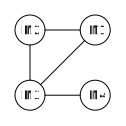
\includegraphics{graphs/movies}\includegraphics{graphs/actors}
\par\end{centering}
\caption{Movies and actors unipartite graphs}
\end{figure}


\subsection{Show that, in general, it is not possible to uniquely reconstruct
a bipartite network from its two unipartite projections}

Here is a counter example constructed from the two unipartite graphs: 

\begin{figure}[H]
\begin{centering}
\includegraphics{graphs/bipartite}
\par\end{centering}
\caption{Counter example \textemdash{} other bipartite network built from the
two unipartite graphs}
\end{figure}


\section{Ensemble averages by enumeration}

\subsection{Calculate, using pen and paper, $\left\langle k\right\rangle $,
$\left\langle C\right\rangle $, and $\left\langle d^{*}\right\rangle $
for $G(N=3,p=1/3)$}

For $N=3$, we have $8$ possible graphs: 
\begin{itemize}
\item 
\begin{multicols}{2}
\begin{itemize}
\item 1 graph with no links 
\item 3 graphs with 1 link
\item 3 graphs with 2 links
\item 1 graph with 3 links
\end{itemize}
\end{multicols}
\end{itemize}
\begin{align*}
\left\langle k\right\rangle  & =\sum_{i=0}^{3}\pi_{i}k\left(G_{i}\right)\\
 & =\left(1-\frac{1}{3}\right)^{3}k\left(G_{0}\right)+3\times\frac{1}{3}\times\left(1-\frac{1}{3}\right)^{2}k\left(G_{1}\right)+3\times\left(\frac{1}{3}\right)^{2}\times\left(1-\frac{1}{3}\right)\times k\left(G_{2}\right)+\left(\frac{1}{3}\right)^{3}k\left(G_{3}\right)\\
 & =\frac{8}{27}\times0+3\times\frac{4}{27}\times\frac{2}{3}+3\times\frac{2}{27}\times\frac{4}{3}+\frac{1}{27}\times\frac{6}{3}\\
 & =\frac{2}{3}
\end{align*}

\begin{align*}
\left\langle C\right\rangle  & =\sum_{i=0}^{3}\pi_{i}C\left(G_{i}\right)\\
 & =\frac{8}{27}\times C\left(G_{0}\right)+\frac{12}{27}\times C\left(G_{1}\right)+\frac{6}{27}\times C\left(G_{2}\right)+\frac{1}{27}\times C\left(G_{3}\right)\\
 & =0+0+0+1\times\frac{1}{27}\\
 & =\frac{1}{27}
\end{align*}

\begin{align*}
\left\langle d^{*}\right\rangle  & =\sum_{i=0}^{3}\pi_{i}d^{*}\left(G_{i}\right)\\
 & =\frac{8}{27}\times d^{*}\left(G_{0}\right)+\frac{12}{27}\times d^{*}\left(G_{1}\right)+\frac{6}{27}\times d^{*}\left(G_{2}\right)+\frac{1}{27}\times d^{*}\left(G_{3}\right)\\
 & =0+\frac{12}{27}\times1+\frac{6}{27}\times2+\frac{1}{27}\times2\\
 & =\frac{25}{27}\approx0,9259
\end{align*}


\subsection{Calculate, using pen and paper, $\left\langle k\right\rangle $,
$\left\langle C\right\rangle $, and $\left\langle d^{*}\right\rangle $
for $G(N=3,p)$}

\begin{align*}
\left\langle k\right\rangle  & =\sum_{i=0}^{3}\pi_{i}k\left(G_{i}\right)\\
 & =\left(1-p\right)^{3}k\left(G_{0}\right)+3p\left(1-p\right)^{2}k\left(G_{1}\right)+3p^{2}\left(1-p\right)k\left(G_{2}\right)+p^{3}k\left(G_{3}\right)\\
 & =2p
\end{align*}

\begin{align*}
\left\langle C\right\rangle  & =\sum_{i=0}^{3}\pi_{i}C\left(G_{i}\right)\\
 & =\left(1-p\right)^{3}C\left(G_{0}\right)+3p\left(1-p\right)^{2}C\left(G_{1}\right)+3p^{2}\left(1-p\right)C\left(G_{2}\right)+p^{3}C\left(G_{3}\right)\\
 & =p^{3}
\end{align*}

\begin{align*}
\left\langle d^{*}\right\rangle  & =\sum_{i=0}^{3}\pi_{i}d^{*}\left(G_{i}\right)\\
 & =\left(1-p\right)^{3}d^{*}\left(G_{0}\right)+3p\left(1-p\right)^{2}d^{*}\left(G_{1}\right)+3p^{2}\left(1-p\right)d^{*}\left(G_{2}\right)+p^{3}d^{*}\left(G_{3}\right)\\
 & =-2p^{3}+3p
\end{align*}

\end{document}
